
% xetex expected
\documentclass[xetex,professionalfont]{beamer}

% we want math
\usepackage{amsmath}

% fixes and extensions to amsmath
\usepackage{mathtools}

% additional math symbols
\usepackage{amssymb}

% good-looking fractions in text via \sfrac
\usepackage{xfrac}

% fix spaces after custom commands (see below for examples)
\usepackage{xspace}

% minted allows for fancy syntax highlighting (requires python with pygments)
% usage:
%   \begin{minted}{python}
%   codeb
%   \end{minted}
\usepackage{minted}

% better looking tables
% usage:
%   begin with a \toprule, write a single row of column headings,
%   then add \midrule and after the columns of data we finish with \bottomrule
% example:
%   \begin{tabular}{llr} \toprule
%   Animal & Description & Price \midrule
%   cat & foo & 10 \\
%   dog & bar & 20 \\ \bottomrule
%   \end{tabular}
% note that good tables generally neither have vertical rules nor double rules
\usepackage{booktabs}

% system font support (requires xetex or luatex)
\usepackage{fontspec}
\setmonofont[Scale=0.7]{Cousine} % part of ttf-chromeos fonts on Arch

% multi-language quotes for babel
\usepackage{csquotes}

% easy way to include copyright information
\usepackage{copyrightbox}

% better bibliographies
\usepackage[backend=biber,style=authoryear]{biblatex}

% language support (english,ngerman)
\usepackage[english]{babel}

% minted screws up line spacings ...
\usepackage{setspace}
\usepackage{enumitem}

\usepackage{pgfplots}

% -----------------------------------------------------------------------------

% specify PDF metadata
\hypersetup{pdftitle={CVSP VO - Object Category Recognition},pdfsubject={},pdfauthor={Christopher Pramerdorfer}}

% copyright font style
\makeatletter\renewcommand{\CRB@setcopyrightfont}{\tiny\color{lightgray}}

% add bib file
\addbibresource{literature.bib}

% use tuwcvl beamer theme
\usetheme{tuwcvl}

% add some space between lines
\setstretch{1.4}

% but not for minted environments
\AtBeginEnvironment{minted}{\singlespacing}

% fix itemize

\setlist{nolistsep}
\setitemize{itemsep=-1mm,label=\usebeamerfont*{itemize item}%
  \usebeamercolor[fg]{itemize item}
  \usebeamertemplate{itemize item}}

\pgfplotsset{width=6.5cm,compat=newest}

\definecolor{darkgreen}{rgb}{0,0.8,0.1}

% -----------------------------------------------------------------------------

% common english abbreviations
\newcommand{\ie}{\mbox{i.e.}\xspace} % i.e.
\newcommand{\eg}{\mbox{e.g.}\xspace} % e.g.

% math - argmin and argmax
\DeclareMathOperator*{\argmin}{arg\,min}
\DeclareMathOperator*{\argmax}{arg\,max}

% shortcuts for number ranges
\newcommand{\NN}{\mathbb{N}}
\newcommand{\ZZ}{\mathbb{Z}}
\newcommand{\QQ}{\mathbb{Q}}
\newcommand{\RR}{\mathbb{R}}

% bold vectors
\renewcommand{\vec}[1]{\ensuremath{\mathbf{#1}}}

% vector shortcuts
\newcommand{\va}{\vec{a}}
\newcommand{\vb}{\vec{b}}
\newcommand{\vc}{\vec{c}}
\newcommand{\ve}{\vec{e}}
\newcommand{\vr}{\vec{r}}
\newcommand{\vs}{\vec{s}}
\newcommand{\vt}{\vec{t}}
\newcommand{\vu}{\vec{u}}
\newcommand{\vv}{\vec{v}}
\newcommand{\vw}{\vec{w}}
\newcommand{\vx}{\vec{x}}
\newcommand{\vy}{\vec{y}}
\newcommand{\vz}{\vec{z}}

\newcommand{\vE}{\vec{E}}
\newcommand{\vF}{\vec{F}}

\newcommand{\bth}{\boldsymbol{\theta}}
\newcommand{\intr}{\boldsymbol{\Lambda}}

% highlight
\newcommand{\highlight}[1]{\textcolor{tuwcvl_inf_red}{\textbf{#1}}}

% make emph red
\let\oldemph\emph
\renewcommand\emph[1]{\textcolor{tuwcvl_inf_red}{#1}}

% -----------------------------------------------------------------------------

\title{Computer Vision Systems Programming VO}
\subtitle{Object Category Recognition}
\author{Christopher Pramerdorfer}
\institute{Computer Vision Lab, Vienna University of Technology}

\begin{document}

% -----------------------------------------------------------------------------

\begin{frame}
\maketitle
\end{frame}

% -----------------------------------------------------------------------------

\begin{frame}
\frametitle{Topics}

Scene classification using the bag of words model \\
Fast face detection using boosted Haar features \\
Convolutional neural networks for large-scale problems

\bigskip
\begin{center}
    \copyrightbox[b]
    {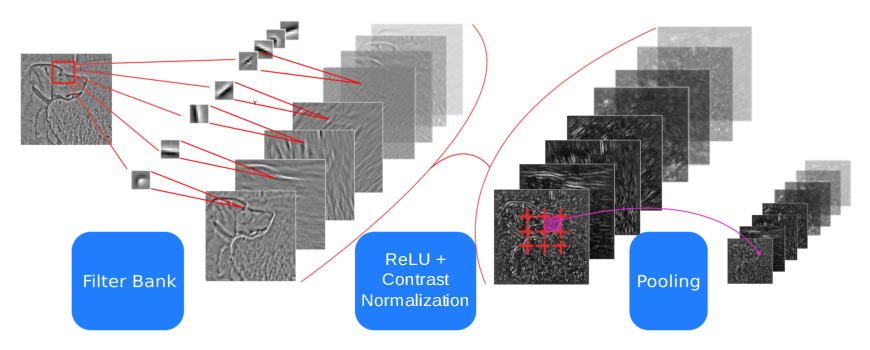
\includegraphics[width=7cm]{figures/cnp-layers.png}}
    {\centering Image adaoted from \cite{kavukcuoglu2011}}
\end{center}

\end{frame}

% -----------------------------------------------------------------------------

\begin{frame}
\frametitle{Scene Classification}
\framesubtitle{Selecting $\vw$}

We want to distinguish between $c$ scene categories
\begin{itemize}
    \item So $w\in\{0,\dots,c-1\}$ (classification problem)
\end{itemize}

\medskip
\begin{center}
    \copyrightbox[b]
    {
\begin{tikzpicture}
    \node[anchor=south west,inner sep=0] (image) at (0,0) {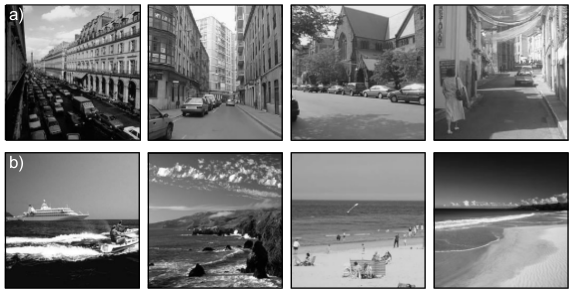
\includegraphics[width=7.75cm]{figures/scene-categories.jpg}};
    \begin{scope}[x={(image.south east)},y={(image.north west)}]
        \node[red] at (-0.13,0.25) {Sea Scenes};
        \node[red] at (-0.15,0.75) {Street Scenes};
    \end{scope}
\end{tikzpicture}
    }
    {\centering Image adapted from \cite{prince12}}
\end{center}

\end{frame}

% -----------------------------------------------------------------------------

\begin{frame}
\frametitle{Scene Classification}
\framesubtitle{Selecting $\vx$}

We represent an image as a collection of \emph{visual words} % this comes from document retrieval - a text consists of words, an image of visual words, so we represent an image by the distribution of its visual words
\begin{itemize}
    \item Images can be compared based on visual word distribution
\end{itemize}

\medskip
\begin{center}
    \copyrightbox[b]
    {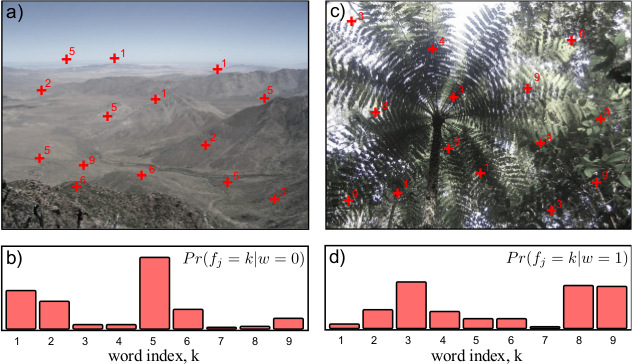
\includegraphics[width=7cm]{figures/visual-words.jpg}} % we see that the visual word representations of these images differ, so they are not of the same class
    {\centering Image from \cite{prince12}}
\end{center}

\end{frame}

% -----------------------------------------------------------------------------

\begin{frame}
\frametitle{Scene Classification}
\framesubtitle{Selecting $\vx$}

Visual words are learned from an image collection
\begin{itemize}
    \item Compute (SIFT) keypoints and descriptors for all images
    \item Cluster descriptors into $k$ clusters using $k$-means % this is the standard method, can use other clustering methods as well
    \item $k$ cluster means represent visual words
\end{itemize}

\medskip
\begin{center}
    \copyrightbox[b]
    {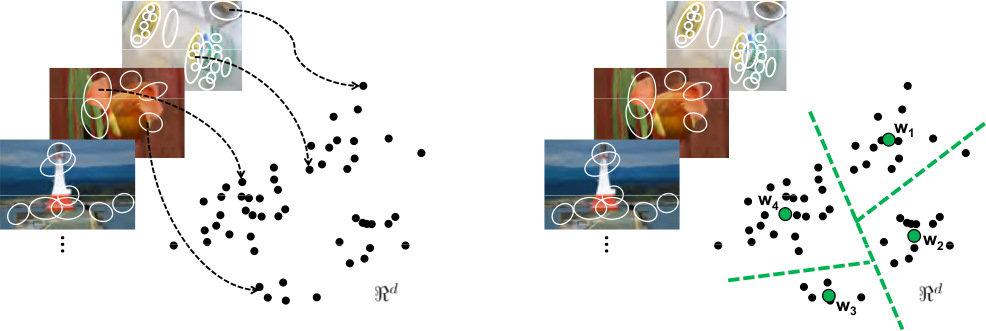
\includegraphics[width=8.5cm]{figures/visual-word-construction.jpg}}
    {\centering Image from \cite{grauman2011}}
\end{center}

\end{frame}

% -----------------------------------------------------------------------------

\begin{frame}
\frametitle{Scene Classification}
\framesubtitle{Selecting $\vx$}

Visual word distribution $\vx\in\NN^k$ of image obtained by
\begin{itemize}
    \item Computing keypoints and descriptors
    \item Assigning each feature to closest visual word % this is again the simplest approach, better performance can be achieved using fuzzy assignment
    \item Summing up the assignment counts for each visual word % and normalizing them of course
\end{itemize}

\medskip
\begin{center}
    \copyrightbox[b]
    {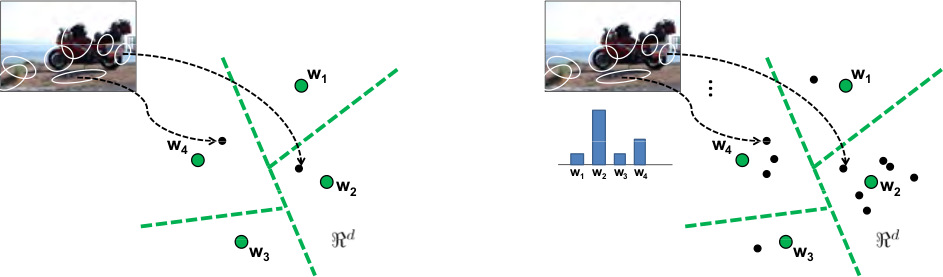
\includegraphics[width=8.5cm]{figures/visual-word-generation.jpg}}
    {\centering Image from \cite{grauman2011}}
\end{center}

\end{frame}

% -----------------------------------------------------------------------------

\begin{frame}
\frametitle{Scene Classification}
\framesubtitle{Selecting $\vx$ and a Model}

This image representation is called \emph{bag of (visual) words}

\bigskip
Now that we have $\vx$ we can select and learn a suitable model
\begin{itemize}
    \item SVMs are often used in the literature
    \item For a probabilistic alternative see \cite{prince12}
\end{itemize}

\end{frame}

% -----------------------------------------------------------------------------

\begin{frame}
\frametitle{Scene Classification}
\framesubtitle{Bag of Visual Words -- Remarks}

Many improvements to this model exist
\begin{itemize}
    \item Better clustering schemes
    \item Fuzzy assignment to visual words
    \item Spatial information (constellation model)
\end{itemize}

\bigskip
Popular and can work well, but no longer state of the art % for this reason, this was quite short, basically in order to make the differences to deep learning clearer

\end{frame}

% -----------------------------------------------------------------------------

\begin{frame}[fragile]
\frametitle{Scene Classification}
\framesubtitle{Bag of Visual Words Using OpenCV}

\footnotesize

\begin{minted}{cpp}
// init SIFT
cv::Ptr<cv::FeatureDetector> kp = cv::FeatureDetector::create("SIFT");
cv::Ptr<cv::DescriptorExtractor> desc = cv::DescriptorExtractor::create("SIFT");

// compute visual words from training data
const int k = 50; // number of visual words
cv::BOWKMeansTrainer trainer(k);

for(const cv::Mat& im : images) { // std::vector of training images
    std::vector<cv::KeyPoint> keypoints; kp->detect(im, keypoints);
    cv::Mat descriptors; desc->compute(im, keypoints, descriptors);
    trainer.add(descriptors);
}

cv::Mat visualWords = trainer.cluster(); // k*128 (SIFT dimension)
\end{minted}

\end{frame}

% -----------------------------------------------------------------------------

\begin{frame}[fragile]
\frametitle{Scene Classification}
\framesubtitle{Bag of Visual Words Using OpenCV}

\footnotesize

\begin{minted}{cpp}
// setup visual word frequency (our x) extractor
cv::Ptr<cv::DescriptorMatcher> fm = cv::makePtr<cv::BFMatcher>(cv::NORM_L2);
cv::BOWImgDescriptorExtractor extractor(desc, fm);
extractor.setVocabulary(visualWords);

// compute x for all training images
cv::Mat xTrain(images.size(), k, CV_32FC1);
for(std::size_t i = 0; i != images.size(); i++) {
    std::vector<cv::KeyPoint> keypoints; kp->detect(images[i], keypoints);
    cv::Mat x; extractor.compute(images[i], keypoints, x);
    xTrain(cv::Rect(0, i, k, 1)) = x;
}

// and corresponding w
cv::Mat wTrain(images.size(), 1, CV_32FC1); // fill me
\end{minted}

\end{frame}

% -----------------------------------------------------------------------------

\begin{frame}[fragile]
\frametitle{Scene Classification}
\framesubtitle{Bag of Visual Words Using OpenCV}

\footnotesize

\begin{minted}{cpp}
// train our model (we use an SVM)
CvSVM svm;
svm.train(xTrain, wTrain);

// now we can predict the class of new images
std::vector<cv::KeyPoint> keypoints; kp->detect(newImage, keypoints);
cv::Mat x; extractor.compute(newImage, keypoints, x);
float w = svm.predict(x); // predicted class label
\end{minted}

\end{frame}

% -----------------------------------------------------------------------------

{
\setbeamertemplate{footline}{}
\begin{frame}

\begin{tikzpicture}[remember picture,overlay]
\fill[white] (current page.north west) rectangle (current page.south east);
\end{tikzpicture}

\end{frame}
}

% -----------------------------------------------------------------------------

\begin{frame}
\frametitle{Face Detection}

\begin{center}
    \copyrightbox[b]
    {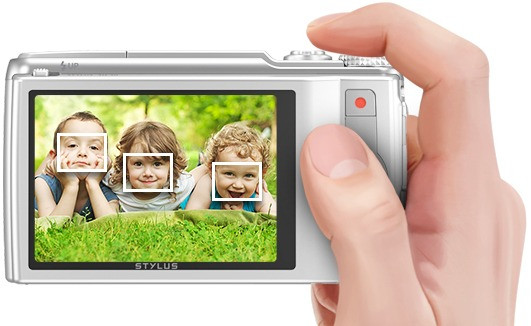
\includegraphics[width=7cm]{figures/camera-faces.jpg}}
    {\centering Image from \url{olympus-europa.com}}
\end{center}

\end{frame}

% -----------------------------------------------------------------------------

\begin{frame}
\frametitle{Face Detection}
\framesubtitle{Selecting $\vw$}

We don't know where the faces are so we % could be 0, could be 10, arbitrary positions
\begin{itemize}
    \item Slide a fixed-size window over the image
    \item Compute $\Pr(w|\vx)$ for each window ($w=1$ if face, 0 if not)
\end{itemize}

\medskip
\begin{center}
\begin{tikzpicture}
\node [inner sep=0pt,above right]{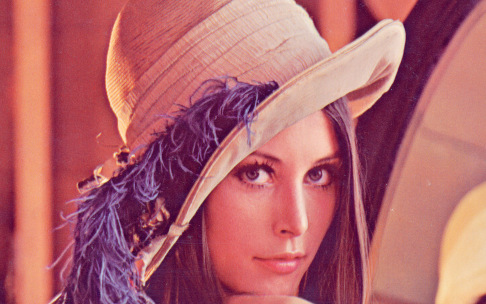
\includegraphics[width=5cm]{figures/lena.jpg}};;
\draw[thick,darkgreen,opacity=0.2] (1.6,0.25) rectangle (3.6,2.25);
\draw[thick,darkgreen,opacity=0.4] (1.7,0.25) rectangle (3.7,2.25);
\draw[thick,darkgreen,opacity=0.6] (1.8,0.25) rectangle (3.8,2.25);
\draw[thick,darkgreen,opacity=0.8] (1.9,0.25) rectangle (3.9,2.25);
\draw[thick,darkgreen] (2,0.25) rectangle (4,2.25);
\end{tikzpicture}
\end{center}

\end{frame}

% -----------------------------------------------------------------------------

\begin{frame}
\frametitle{Face Detection}
\framesubtitle{Selecting $\vx$}

Which are good features for this task?

\bigskip
Must be fast to compute (many windows) \\
Must be robust to illumination, so we use gradient information % because we assume a general unconstrained setting

\bigskip
Different approaches to encoding gradient information
\begin{itemize}
    \item Compute gradients, pool orientations in blocks (e.g.\ SIFT) % weighted by magnitude
    \item Use a collection of Gabor filters % we briefly covered those in an earlier lecture
\end{itemize}

\end{frame}

% -----------------------------------------------------------------------------

\begin{frame}
\frametitle{Face Detection}
\framesubtitle{Selecting $\vx$}

We want something faster
\begin{itemize}
    \item So we use a \enquote{blocky} approximation of Gabor filters
    \item Difference between rectangular subwindows (\emph{Haar features})
    \item Can be computed in constant time using integral images
\end{itemize}

\medskip
\begin{center}
    \copyrightbox[b]
    {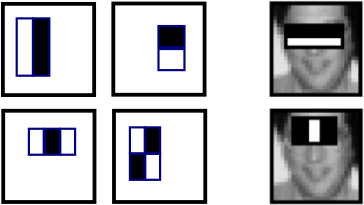
\includegraphics[width=5cm]{figures/haar-features.png}}
    {\centering Image adapted from \cite{prince12}}
\end{center}

\end{frame}

% -----------------------------------------------------------------------------

\begin{frame}
\frametitle{Face Detection}
\framesubtitle{Selecting $\vx$}

Computing a Haar feature at a location yields a scalar $f_i$ \\
We define $\vx=(x_1,\dots,x_I)$ with $x_i=\text{heaviside}(f_i-t_i)$ % heaviside step function returns 0 if f_i-t_i < 0, else 1

\bigskip
$I$ is very large
\begin{itemize}
    \item Different Haar features, subwindow locations, $t_i$
    \item We thus learn which features $x_i$ work best
\end{itemize}

\end{frame}

% -----------------------------------------------------------------------------

\begin{frame}
\frametitle{Face Detection}
\framesubtitle{Model Selection and Learning}

We model $\Pr(w|\vx)$ as a weighted sum of a feature subset
\[
    \Pr(w|\vx) \propto a = \phi_0+\sum_k \phi_k\, x_k \qquad (1\leq k\leq I)
\]
And learn the parameters $\bth=(\phi_0,\phi_k,x_k)$ from training samples
\begin{itemize}
    \item For each $x_k$ in a large precomputed set
    \item Find optimal $\phi_0,\phi_k$
    \item Add best $x_k$ (and $\phi_0,\phi_k$) to sum and repeat
\end{itemize}

\bigskip
This incremental approach is called \emph{boosting}

\end{frame}

% -----------------------------------------------------------------------------

\begin{frame}
\frametitle{Face Detection}
\framesubtitle{Learning and Inference}

We stop adding features at some point
\begin{itemize}
    \item If the classification error no longer decreases significantly
    \item After a specified maximum number of iterations
\end{itemize}

\bigskip
We end up with $K$ good features, $K\ll I$
\begin{itemize}
    \item For prediction we compute only these $K$ features
    \item Stop early if $P(w=0)>t$ after processing $J\ll K$ features % this is optional and inaccurate but makes detection extremely fast as we only have to compute a few features for non-face regions
\end{itemize}

\end{frame}

% -----------------------------------------------------------------------------

\begin{frame}
\frametitle{Face Detection}
\framesubtitle{Learning and Inference}

If we don't care about probabilities, we choose $w=\text{heaviside}(a)$

\bigskip
If we do, we use \emph{logistic regression}, $\Pr(w|\vx)=\text{Bern}_w(\text{sig}(a))$
\begin{itemize}
    \item We model $w$ as a Bernoulli distribution
    \item Pass $a$ through a logistic sigmoid to map it to $[0,1]$
    \item Called \emph{logitboost} in this context
\end{itemize}

\end{frame}

% -----------------------------------------------------------------------------

\begin{frame}
\frametitle{Face Detection}
\framesubtitle{Remarks}

This method was proposed in \cite{viola2001} \\
Very efficient, ideal for e.g.\ digital cameras

\bigskip
Trades off efficiency for accuracy
\begin{itemize}
    \item Features capture gradients coarsely, no color information
    \item More powerful but slower methods exist
\end{itemize}

\bigskip
Not invariant to scale changes (fixed-size window)
\begin{itemize}
    \item Repeat detection at different image scales
\end{itemize}

\end{frame}

% -----------------------------------------------------------------------------

\begin{frame}[fragile]
\frametitle{Face Detection}
\framesubtitle{Viola \& Jones Face Detector in OpenCV}

Detect faces using a pretrained model \\
OpenCV also supports training

\bigskip
\small
\begin{minted}{python}
# detect faces using a pretrained cascade
image = cv2.imread('faces.jpg', cv2.IMREAD_GRAYSCALE)
cascade = cv2.CascadeClassifier('haarcascade_frontalface_default.xml')
faces = cascade.detectMultiScale(image) # should tune parameters
\end{minted}

\end{frame}

% -----------------------------------------------------------------------------

{
\setbeamertemplate{footline}{}
\begin{frame}

\begin{tikzpicture}[remember picture,overlay]
\fill[white] (current page.north west) rectangle (current page.south east);
\end{tikzpicture}

\end{frame}
}

% -----------------------------------------------------------------------------

\begin{frame}
\frametitle{Deep Learning}
\framesubtitle{Motivation}

Selecting good features $\vx$ for object recognition is challenging
\begin{itemize}
    \item Why we previously learned $\vx$
\end{itemize}

\bigskip
Learned features were low-level
\begin{itemize}
    \item Based on SIFT descriptors or Haar wavelets
\end{itemize}

\bigskip
We want task-specific high-level features
\begin{itemize}
    \item Virtually impossible to design manually
    \item So we learn them as well
\end{itemize}

\end{frame}

% -----------------------------------------------------------------------------

\begin{frame}
\frametitle{Deep Learning}
\framesubtitle{Motivation}

We learn these features hierarchically
\begin{itemize}
    \item Model consists of layers
    \item The higher up the layer, the higher-level the feature
    \item Features in layer $n$ are based on those in layer $n-1$
    \item Results in a \textit{deep} model, hence \emph{deep learning}
\end{itemize}

\bigskip
At the same time we learn to predict $\vw$

\end{frame}

% -----------------------------------------------------------------------------

\begin{frame}
\frametitle{Deep Learning}
\framesubtitle{Motivation}

\begin{center}
    \copyrightbox[b]
    {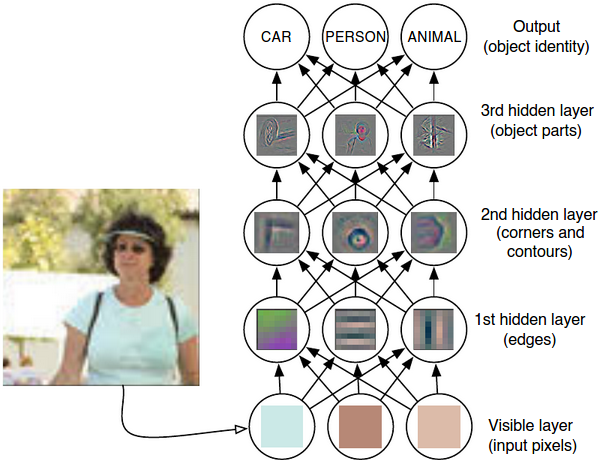
\includegraphics[width=7cm]{figures/dl-layer-example}}
    {\centering Image from \cite{bengio2015}}
\end{center}

\end{frame}

% -----------------------------------------------------------------------------

\begin{frame}
\frametitle{Deep Learning}
\framesubtitle{Convolutional Neural Networks}

Deep model optimized for images
\begin{itemize}
    \item Exploits correlations between adjacent pixels
    \item Performs remarkably well in many recognition tasks
\end{itemize}

\bigskip
\begin{center}
    \enquote{From now on, deep learning has to be considered as the primary\\ candidate in essentially any visual recognition task}\\
    ~ [\cite{razavian14}] % check out this paper. also see Pierre Sermanet's slides for a good overview of how DL has advanced the state of the art in many fields, available here: https://sites.google.com/site/deeplearningcvpr2014/
\end{center}

\end{frame}

% -----------------------------------------------------------------------------

\begin{frame}
\frametitle{Deep Learning}
\framesubtitle{Structure of Convolutional Neural Networks}

\emph{Multilayer Perceptrons} (\emph{MLPs}) with some twists

\bigskip
\begin{center}
    \copyrightbox[b]
    {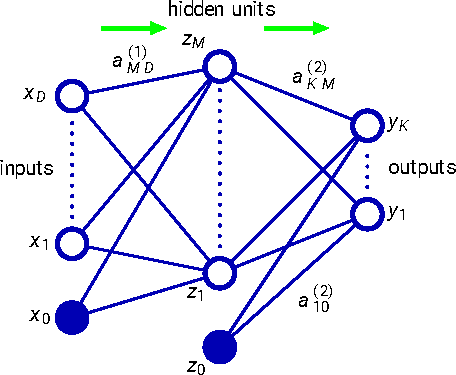
\includegraphics[width=5cm]{figures/two-layer-mlp.pdf}}
    {\centering Image adapted from \cite{bishop2006}}
\end{center}

\end{frame}

% -----------------------------------------------------------------------------

\begin{frame}
\frametitle{Deep Learning}
\framesubtitle{Multilayer Perceptrons}

Remember the \emph{Perceptron}?
\begin{itemize}
    \item Model for binary classification, $w=\text{heaviside}(\va^\top\vx+b)$
    \item Parameters $\bth=(\va,b)$ learned from data % the decision hyperplane is wx+b=0
\end{itemize}

\bigskip
Limitations
\begin{itemize}
    \item Linear decision boundaries
    \item Only two classes, not probabilistic
    \item Learning never converges for non-separable data
\end{itemize}

\end{frame}

% -----------------------------------------------------------------------------

\begin{frame}
\frametitle{Deep Learning}
\framesubtitle{Multilayer Perceptrons}

To overcome these limitations we
\begin{itemize}
    \item Replace step function with continuous $f$ (e.g.\ tanh)
    \item Add a layer of $M$ such \enquote{Perceptrons} (\emph{hidden units})
    \item Add $K$ \emph{output units} (number of classes)
\end{itemize}

\medskip
\begin{center}
    \copyrightbox[b]
    {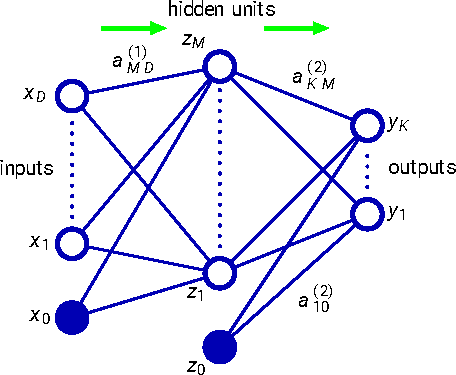
\includegraphics[width=4cm]{figures/two-layer-mlp.pdf}}
    {\centering Image adapted from \cite{bishop2006}}
\end{center}

\end{frame}

% -----------------------------------------------------------------------------

\begin{frame}
\frametitle{Deep Learning}
\framesubtitle{Multilayer Perceptrons}

Output of $m$th hidden unit is $z_m(\vx)=f(\va_m^\top\,\vx)$
\begin{itemize}
    \item Bias $b$ included in $\va$ and $\vx$, $a_0=b$, $x_0=1$
\end{itemize}

\bigskip
\begin{center}
    \copyrightbox[b]
    {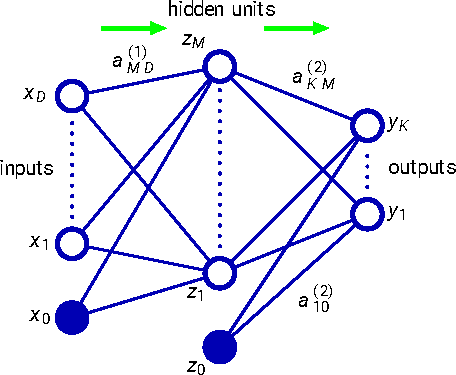
\includegraphics[width=4.5cm]{figures/two-layer-mlp.pdf}}
    {\centering Image from \cite{bishop2006}}
\end{center}

\end{frame}

% -----------------------------------------------------------------------------

\begin{frame}
\frametitle{Deep Learning}
\framesubtitle{Multilayer Perceptrons}

Output of $k$th output unit is $y_k(\vz)=g(\va_k^\top\,\vz)$ % this again includes the bias
\begin{itemize}
    \item $g$ depends on problem (regression, classification) % identity for regression, softmax for classification; must be differentiable
\end{itemize}

\bigskip
\begin{center}
    \copyrightbox[b]
    {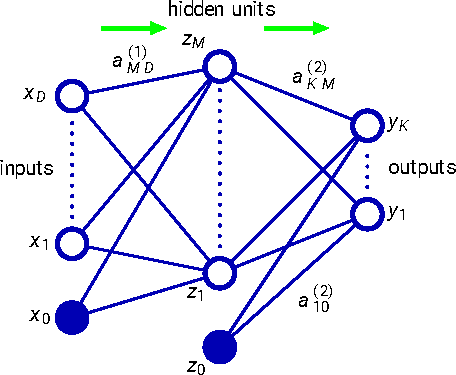
\includegraphics[width=4.5cm]{figures/two-layer-mlp.pdf}}
    {\centering Image from \cite{bishop2006}}
\end{center}

\end{frame}

% -----------------------------------------------------------------------------

\begin{frame}
\frametitle{Deep Learning}
\framesubtitle{Multilayer Perceptrons}

Both $f$ and $g$ are differentiable
\begin{itemize}
    \item Learn parameters using gradient descent % here a contains all weights / the error function to minimize depends on the task; for regression we minimize the sum of squared residuals
    \item Gradients evaluated via error backpropagation % no details here, check bishop2006, for example
\end{itemize}

\bigskip
Properties
\begin{itemize}
    \item Powerful, can approximate any decision boundary if $M$ is large
    \item Does not scale to images due to full connectivity
    \item Not deep (not possible due to scaling issues)
\end{itemize}

\end{frame}

% -----------------------------------------------------------------------------

\begin{frame}
\frametitle{Deep Learning}
\framesubtitle{Multilayer Perceptrons}

\begin{center}
\copyrightbox[b]
{
\begin{tikzpicture}
    \node[anchor=south west,inner sep=0] (image) at (0,0) {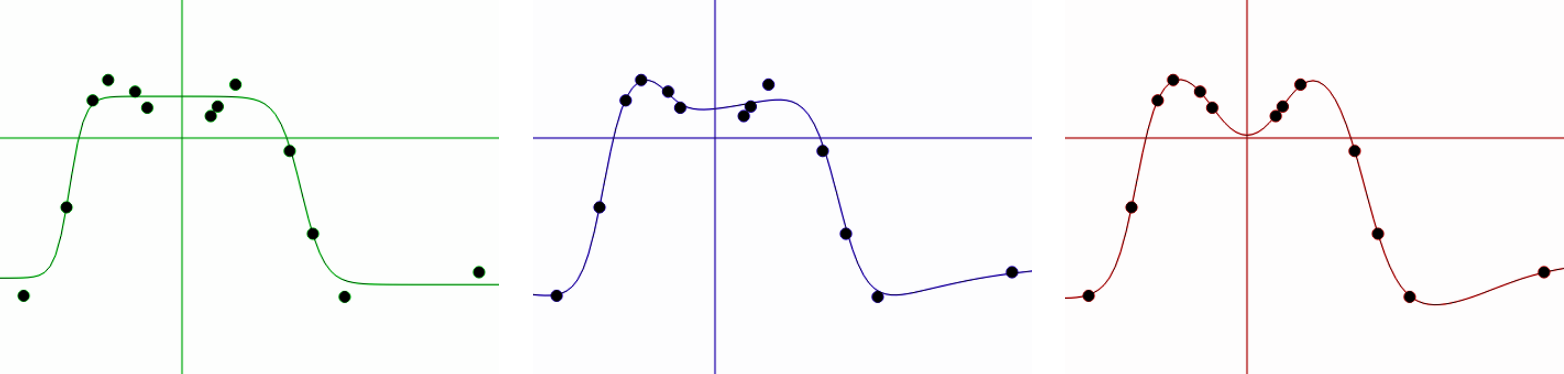
\includegraphics[width=11cm]{figures/mlp-fitting.png}};
    \begin{scope}[x={(image.south east)},y={(image.north west)}]
        \node at (0.167,0.1) {\small $M=2$};
        \node at (0.51,0.1) {\small $M=5$};
        \node at (0.855,0.1) {\small $M=20$};
    \end{scope}
\end{tikzpicture}
}
{\centering Image adapted from \href{http://cs.stanford.edu/people/karpathy/convnetjs/demo/regression.html}{\texttt{cs.stanford.edu/people/karpathy/convnetjs/}}}
\end{center}

\end{frame}

% -----------------------------------------------------------------------------

\begin{frame}
\frametitle{Deep Learning}
\framesubtitle{Multilayer Perceptrons}

QVGA image ($D=76800$), $M=500$ : $\sim 38$m parameters

\bigskip
\begin{center}
\begin{tikzpicture}
    \node[anchor=south west,inner sep=0] (image) at (0,0) {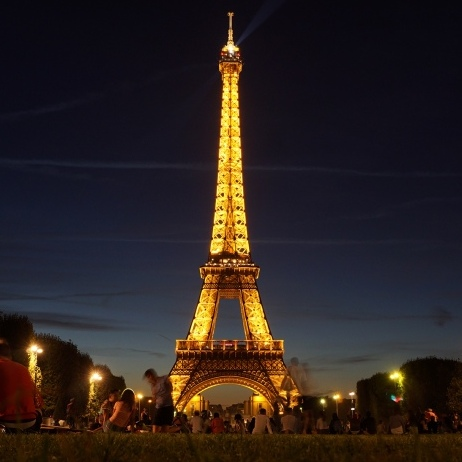
\includegraphics[width=4.5cm]{figures/eiffel-tower.jpg}};
    \begin{scope}[x={(image.south east)},y={(image.north west)}]
        \draw[step=0.02, gray] (0,0) grid (1.001,1.001);
        \foreach \x in {0.01,0.05,...,1} {
            \foreach \y in {0.01,0.05,...,1} {
                \draw[blue,opacity=0.33] (\x,\y) -- (1.3, 0.5);
            }
        }
        \foreach \x in {0.1,0.2,...,0.8} {
            \draw[blue,thick,fill=white] (1.3,\x) circle (0.05cm);
        }
        \node at (1.3,0.9) {$M$};
    \end{scope}
\end{tikzpicture}
\end{center}

\end{frame}

% -----------------------------------------------------------------------------

\begin{frame}
\frametitle{Deep Learning}
\framesubtitle{Convolutional Layers}

Nearby pixels are closely correlated, the rest is not % because they depict totally different objects (parts)
\begin{itemize}
    \item We use $D$ hidden units (one per input pixel) % we don't need to, but this is common
    \item Connect each only to nearby pixels (\emph{local receptive field})
\end{itemize}

\medskip
\begin{center}
\begin{tikzpicture}
    \node[anchor=south west,inner sep=0] (image) at (0,0) {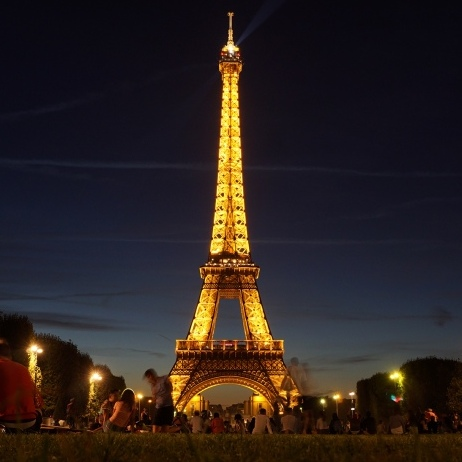
\includegraphics[width=4cm]{figures/eiffel-tower.jpg}};
    \begin{scope}[x={(image.south east)},y={(image.north west)}]
    \draw[step=0.02, gray] (0,0) grid (1.001,1.001);
    \draw[step=0.02, gray] (1.2,0) grid (2.201,1.001);
    %
    \draw[draw=none,fill=blue] (1.54,0.34) rectangle (1.56,0.36);
    \draw[step=0.02, blue] (0.3,0.3) grid (0.401,0.401);
    \foreach \x in {0.31,0.33,...,0.4} {
        \foreach \y in {0.31,0.33,...,0.4} {
            \draw[blue,opacity=0.33] (\x,\y) -- (1.55, 0.35);
        }
    }
    %
    \draw[draw=none,fill=red] (1.34,0.84) rectangle (1.36,0.86);
    \draw[step=0.02, red] (0.1,0.8) grid (0.201,0.901);
    \foreach \x in {0.11,0.13,...,0.2} {
        \foreach \y in {0.81,0.83,...,0.9} {
            \draw[red,opacity=0.33] (\x,\y) -- (1.35, 0.85);
        }
    }
    %
    \draw[draw=none,fill=darkgreen] (2.04, 0.64) rectangle (2.06, 0.66);
    \draw[step=0.02, darkgreen] (0.8,0.6) grid (0.901,0.701);
    \foreach \x in {0.81,0.83,...,0.9} {
        \foreach \y in {0.61,0.63,...,0.7} {
            \draw[darkgreen,opacity=0.33] (\x,\y) -- (2.05, 0.65);
        }
    }
    \end{scope}
\end{tikzpicture}
\end{center}

\end{frame}

% -----------------------------------------------------------------------------

\begin{frame}
\frametitle{Deep Learning}
\framesubtitle{Convolutional Layers}

$M$ much higher but much fewer parameters
\begin{itemize}
    \item $\sim 2$m in example with $5\times5$ receptive field
\end{itemize}

\medskip
\begin{center}
\begin{tikzpicture}
    \node[anchor=south west,inner sep=0] (image) at (0,0) {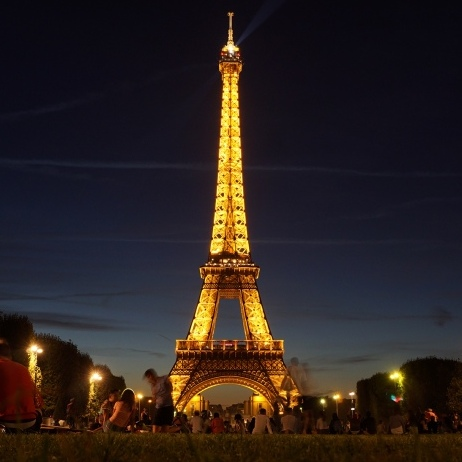
\includegraphics[width=4cm]{figures/eiffel-tower.jpg}};
    \begin{scope}[x={(image.south east)},y={(image.north west)}]
    \draw[step=0.02, gray] (0,0) grid (1.001,1.001);
    \draw[step=0.02, gray] (1.2,0) grid (2.201,1.001);
    %
    \draw[draw=none,fill=blue] (1.54,0.34) rectangle (1.56,0.36);
    \draw[step=0.02, blue] (0.3,0.3) grid (0.401,0.401);
    \foreach \x in {0.31,0.33,...,0.4} {
        \foreach \y in {0.31,0.33,...,0.4} {
            \draw[blue,opacity=0.33] (\x,\y) -- (1.55, 0.35);
        }
    }
    %
    \draw[draw=none,fill=red] (1.34,0.84) rectangle (1.36,0.86);
    \draw[step=0.02, red] (0.1,0.8) grid (0.201,0.901);
    \foreach \x in {0.11,0.13,...,0.2} {
        \foreach \y in {0.81,0.83,...,0.9} {
            \draw[red,opacity=0.33] (\x,\y) -- (1.35, 0.85);
        }
    }
    %
    \draw[draw=none,fill=darkgreen] (2.04, 0.64) rectangle (2.06, 0.66);
    \draw[step=0.02, darkgreen] (0.8,0.6) grid (0.901,0.701);
    \foreach \x in {0.81,0.83,...,0.9} {
        \foreach \y in {0.61,0.63,...,0.7} {
            \draw[darkgreen,opacity=0.33] (\x,\y) -- (2.05, 0.65);
        }
    }
    \end{scope}
\end{tikzpicture}
\end{center}

\end{frame}

% -----------------------------------------------------------------------------

\begin{frame}
\frametitle{Deep Learning}
\framesubtitle{Convolutional Layers}

Learned features should work well everywhere in the image
\begin{itemize}
    \item We don't know where objects will be
\end{itemize}

\bigskip
So we define that all hidden units must have \textit{same} weights
\begin{itemize}
    \item Number of parameters now independent of $M$ % only 26 in example, 5*5 + 1 for bias
    \item But we now can learn only a single feature
\end{itemize}

\bigskip
So we duplicate the hidden layer $F$ times
\begin{itemize}
    \item Each duplicate (\emph{feature map}) learns a feature
\end{itemize}

\end{frame}

% -----------------------------------------------------------------------------

\begin{frame}
\frametitle{Deep Learning}
\framesubtitle{Convolutional Layers}

$F=100$, $5\times5$ receptive field : $\sim 2600$ parameters

\medskip
\begin{center}
\begin{tikzpicture}
    \node[anchor=south west,inner sep=0] (image) at (0,0) {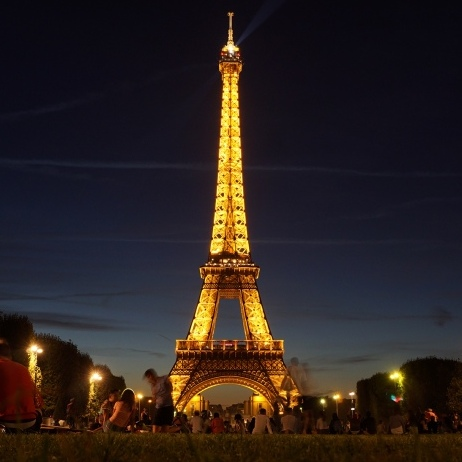
\includegraphics[width=4cm]{figures/eiffel-tower.jpg}};
    \begin{scope}[x={(image.south east)},y={(image.north west)}]
    \draw[step=0.02, gray] (0,0) grid (1.001,1.001);
    \draw[step=0.02, red, opacity=0.33] (1.2,0.0) grid (2.201,1.001);
    \draw[step=0.02, darkgreen, opacity=0.33] (1.3,0.1) grid (2.301,1.101);
    \draw[step=0.02, blue, opacity=0.33] (1.4,0.2) grid (2.401,1.201);
    \draw[step=0.02, white] (0.04,0.04) grid (0.141,0.141);
    %
    \draw[draw=none,fill=red] (1.28, 0.08) rectangle (1.30, 0.1);
    \foreach \x in {0.05,0.07,...,0.14} {
        \foreach \y in {0.05,0.07,...,0.14} {
            \draw[red,opacity=0.33] (\x,\y) -- (1.29, 0.09);
        }
    }
    %
    \draw[draw=none,fill=darkgreen] (1.38, 0.18) rectangle (1.40, 0.2);
    \foreach \x in {0.05,0.07,...,0.14} {
        \foreach \y in {0.05,0.07,...,0.14} {
            \draw[darkgreen,opacity=0.33] (\x,\y) -- (1.39, 0.19);
        }
    }
    %
    \draw[draw=none,fill=blue] (1.48, 0.28) rectangle (1.50, 0.3);
    \foreach \x in {0.05,0.07,...,0.14} {
        \foreach \y in {0.05,0.07,...,0.14} {
            \draw[blue,opacity=0.33] (\x,\y) -- (1.49, 0.29);
        }
    }
    %
    \node at (2.25,0.0) {\small $1$};
    \node at (2.38,0.1) {\small $\cdots$};
    \node at (2.45,0.2) {\small $F$};
    \end{scope}
\end{tikzpicture}
\end{center}

\end{frame}

% -----------------------------------------------------------------------------

\begin{frame}
\frametitle{Deep Learning}
\framesubtitle{Convolutional Layers}

Such layers are called \emph{convolutional (conv) layers}
\begin{itemize}
    \item Feature map evaluation equals convolution with kernel $\va$
    \item Followed by $f$ (often $f(\cdot)=\max(0,\cdot)$ (ReLU))
\end{itemize}

\bigskip
Few parameters, so we can stack conv layers (deep network)
\begin{itemize}
    \item Conv layer $n$ operates on feature maps in layer $n-1$ % on all or a subset 
    \item Learns features by combining those learned in layer $n-1$ % corresponds to a 3D convolution
\end{itemize}

% \bigskip
% MLPs with such layers are \emph{Convolutional Neural Networks} (\emph{CNNs})

\end{frame}

% -----------------------------------------------------------------------------

\begin{frame}
\frametitle{Deep Learning}
\framesubtitle{Convolutional Layers}

\begin{center}
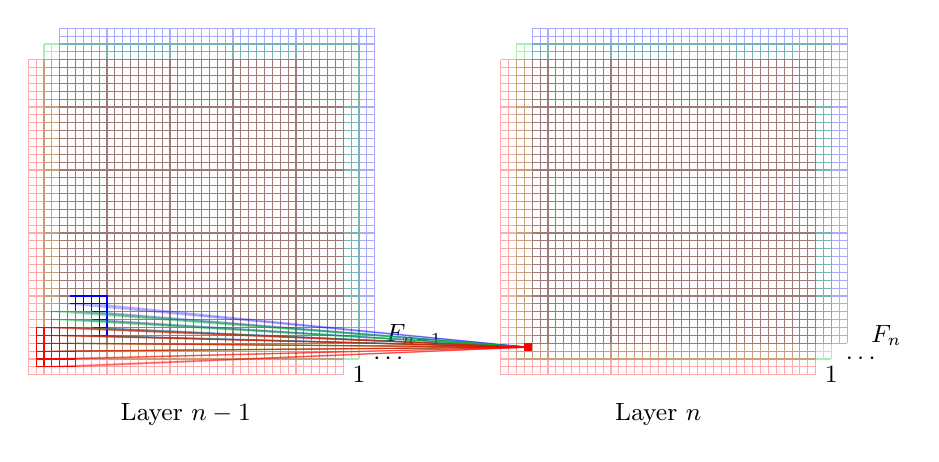
\begin{tikzpicture}
\draw[step=0.1, blue, opacity=0.33] (0.4,0.4) grid (4.401,4.401);
\draw[step=0.1, darkgreen, opacity=0.33] (0.2,0.2) grid (4.201,4.201);
\draw[step=0.1, red, opacity=0.33] (0.0,0.0) grid (4.001,4.001);
%
\node at (2,-0.5) {\small Layer $n-1$};
\node at (4.2,0.0) {\small $1$};
\node at (4.6,0.2) {\small $\cdots$};
\node at (4.9,0.5) {\small $F_{n-1}$};
%
\draw[step=0.1, blue, opacity=0.33] (6.4,0.4) grid (10.401,4.401);
\draw[step=0.1, darkgreen, opacity=0.33] (6.2,0.2) grid (10.201,4.201);
\draw[step=0.1, red, opacity=0.33] (6.0,0.0) grid (10.001,4.001);
%
\node at (8,-0.5) {\small Layer $n$};
\node at (10.2,0.0) {\small $1$};
\node at (10.6,0.2) {\small $\cdots$};
\node at (10.9,0.5) {\small $F_{n}$};
%
\draw[step=0.1, blue] (0.53,0.5) grid (1.01,1.01);
\foreach \x in {0.5,0.6,...,1.0} {
    \foreach \y in {0.5,0.6,...,1.0} {
        \draw[blue,opacity=0.2] (\x,\y) -- (6.35, 0.35);
    }
}
%
\draw[step=0.1, darkgreen] (0.3,0.3) grid (0.81,0.81);
\foreach \x in {0.3,0.4,...,0.8} {
    \foreach \y in {0.3,0.4,...,0.8} {
        \draw[darkgreen,opacity=0.2] (\x,\y) -- (6.35, 0.35);
    }
}
%
\draw[step=0.1, red] (0.1,0.1) grid (0.61,0.61);
\foreach \x in {0.1,0.2,...,0.6} {
    \foreach \y in {0.1,0.2,...,0.6} {
        \draw[red,opacity=0.2] (\x,\y) -- (6.35, 0.35);
    }
}
%
\draw[draw=none,fill=red] (6.3, 0.3) rectangle (6.4, 0.4);
\end{tikzpicture}
\end{center}

\end{frame}

% -----------------------------------------------------------------------------

\begin{frame}
\frametitle{Deep Learning}
\framesubtitle{Pooling Layers}

Most CNNs also contain \emph{pooling layers}
\begin{itemize}
    \item Pool (aggregate) information locally (e.g.\ max, mean)
    \item Reduces data size, robustness to small object movement
\end{itemize}

\medskip
\begin{center}
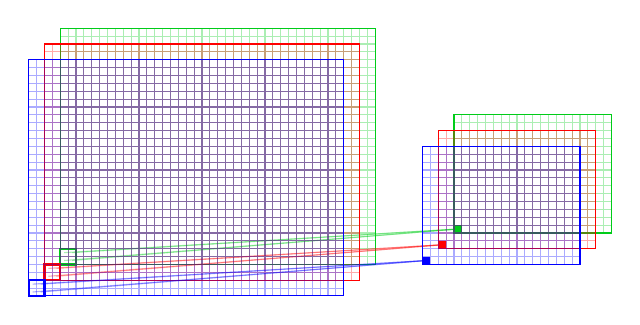
\begin{tikzpicture}
% darkgreen
\draw[step=1mm,darkgreen,opacity=0.33] (0.4,0.4) grid (4.4,3.4);
\draw[darkgreen] (0.4,0.4) rectangle (4.4,3.4);
%
\draw[step=1mm,darkgreen,opacity=0.33] (5.4,0.8) grid (7.4,2.3);
\draw[darkgreen] (5.4,0.8) rectangle (7.4,2.3);
%
\draw[darkgreen,thick] (0.4,0.4) rectangle (0.6,0.6);
\draw[draw=none,fill=darkgreen] (5.4,0.8) rectangle (5.5,0.9);
\draw[darkgreen,opacity=0.33] (0.45,0.45) -- (5.45, 0.85);
\draw[darkgreen,opacity=0.33] (0.55,0.45) -- (5.45, 0.85);
\draw[darkgreen,opacity=0.33] (0.45,0.55) -- (5.45, 0.85);
\draw[darkgreen,opacity=0.33] (0.55,0.55) -- (5.45, 0.85);
%
% red
%
\draw[step=1mm,red,opacity=0.33] (0.2,0.2) grid (4.2,3.2);
\draw[red] (0.2,0.2) rectangle (4.2,3.2);
%
\draw[step=1mm,red,opacity=0.33] (5.2,0.6) grid (7.2,2.1);
\draw[red] (5.2,0.6) rectangle (7.2,2.1);
%
\draw[red,thick] (0.2,0.2) rectangle (0.4,0.4);
\draw[draw=none,fill=red] (5.2,0.6) rectangle (5.3,0.7);
\draw[red,opacity=0.33] (0.25,0.25) -- (5.25, 0.65);
\draw[red,opacity=0.33] (0.35,0.25) -- (5.25, 0.65);
\draw[red,opacity=0.33] (0.25,0.35) -- (5.25, 0.65);
\draw[red,opacity=0.33] (0.35,0.35) -- (5.25, 0.65);
%
% blue
%
\draw[step=1mm,blue,opacity=0.33] (0,0) grid (4,3);
\draw[blue] (0,0) rectangle (4,3);
%
\draw[step=1mm,blue,opacity=0.33] (5,0.4) grid (7,1.9);
\draw[blue] (5,0.4) rectangle (7,1.9);
%
\draw[blue,thick] (0,0) rectangle (0.2,0.2);
\draw[draw=none,fill=blue] (5,0.4) rectangle (5.1,0.5);
\draw[blue,opacity=0.33] (0.05,0.05) -- (5.05, 0.45);
\draw[blue,opacity=0.33] (0.15,0.05) -- (5.05, 0.45);
\draw[blue,opacity=0.33] (0.05,0.15) -- (5.05, 0.45);
\draw[blue,opacity=0.33] (0.15,0.15) -- (5.05, 0.45);
\end{tikzpicture}
\end{center}

\end{frame}

% -----------------------------------------------------------------------------

\begin{frame}
\frametitle{Deep Learning}
\framesubtitle{Convolutional Neural Networks}

\emph{Convolutional Neural Networks} (\emph{CNNs}) consist of
\begin{itemize}
    \item One or several conv layers (and others)
    \item Followed by a traditional MLP operating on learned features
\end{itemize}

\medskip
\begin{center}
    \copyrightbox[b]
    {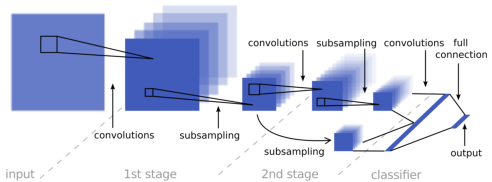
\includegraphics[width=8cm]{figures/convnet.pdf}}
    {\centering Image adapted from \cite{sermanet2012}} % this net is a bit more complicated because it has skip connections
\end{center}

\end{frame}

% -----------------------------------------------------------------------------

\begin{frame}
\frametitle{Deep Learning}
\framesubtitle{Convolutional Neural Networks Learn High-Level Features}

\begin{center}
    \copyrightbox[b]
    {
\begin{tikzpicture}
    \node[anchor=south west,inner sep=0] (image) at (0,0) {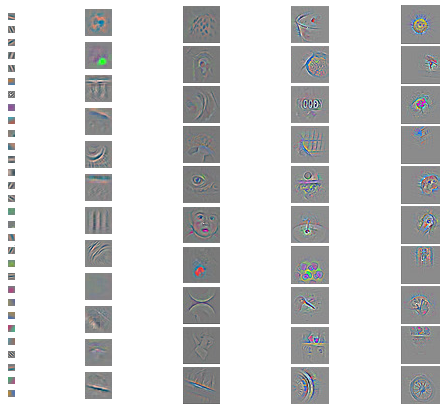
\includegraphics[width=6.5cm]{figures/cnn-features.png}};
    \begin{scope}[x={(image.south east)},y={(image.north west)}]
    \node [rotate=90] at (-0.02,0.5) {\small Layer 1};
    \node [rotate=90] at (0.15,0.5) {\small Layer 2};
    \node [rotate=90] at (0.37,0.5) {\small Layer 3};
    \node [rotate=90] at (0.61,0.5) {\small Layer 4};
    \node [rotate=90] at (0.86,0.5) {\small Layer 5};
    \end{scope}
\end{tikzpicture}
    }
    {\centering Image adapted from \cite{zeiler2014}}
\end{center}

\end{frame}

% -----------------------------------------------------------------------------

\begin{frame}
\frametitle{Deep Learning}
\framesubtitle{Convolutional Neural Networks}

CNNs were proposed long ago
\begin{itemize}
    \item \cite{lecun1989} : Zip code recognition using a CNN
\end{itemize}

\bigskip
Large, deep CNNs possible now
\begin{itemize}
    \item Powerful and flexible GPUs
    \item Large datasets to avoid overfitting (e.g.\ ImageNet)
\end{itemize}

\end{frame}

% -----------------------------------------------------------------------------

\begin{frame}
\frametitle{Deep Learning}
\framesubtitle{Applications -- Zip Code Recognition}

Simple CNN for Zip Code Recognition
\begin{itemize}
    \item Using ConvNetJS (Java Script library)
    \item \href{http://cs.stanford.edu/people/karpathy/convnetjs/demo/mnist.html}{\texttt{cs.stanford.edu/people/karpathy/convnetjs/demo/mnist.html}}
\end{itemize}

\bigskip
\begin{center}
    \copyrightbox[b]
    {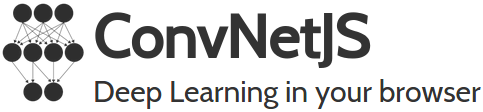
\includegraphics[width=5cm]{figures/convnetjs-logo.png}}
    {\centering Image from \url{convnetjs.com}}
\end{center}

\end{frame}

% -----------------------------------------------------------------------------

\begin{frame}
\frametitle{Deep Learning}
\framesubtitle{Applications -- Face Recognition by \cite{taigman2013}}

Face recognition via 3D face alignment and CNNs
\begin{itemize}
    \item conv $\Rightarrow$ pooling $\Rightarrow$ conv for low-level features
    \item Locally connected layers for high-level features % these are conv layers without weight sharing, hence the large number of parameters. weight sharing is not used here because features differ between face regions (faces are aligned)
    % \item $\sim120$ million parameters, $~\sim4$ million training images
    \item Human-level face verification performance % more recent nets even surpass humans
\end{itemize}

\bigskip
\begin{center}
    \copyrightbox[b]
    {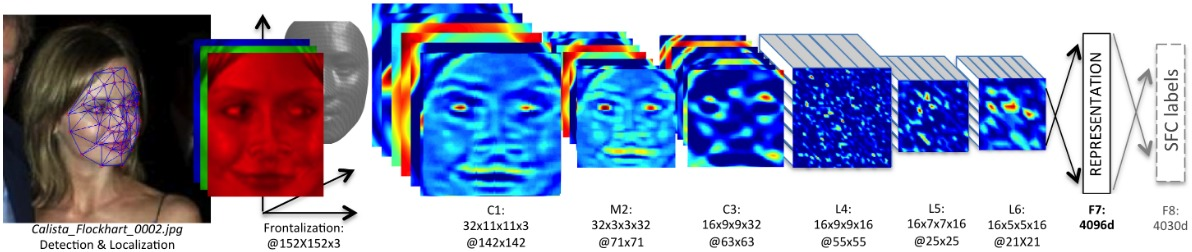
\includegraphics[width=10cm]{figures/deepface-net.jpg}}
    {\centering Image from \cite{taigman2013}}
\end{center}

\end{frame}

% -----------------------------------------------------------------------------

\begin{frame}
\frametitle{Deep Learning}
\framesubtitle{Applications -- Object Recognition}

Object recognition on the ImageNet database
\begin{itemize}
    \item $\sim14$ million images categorized hierarchically
    \item Annual object recognition challenges
\end{itemize}

\begin{center}
    \copyrightbox[b]
    {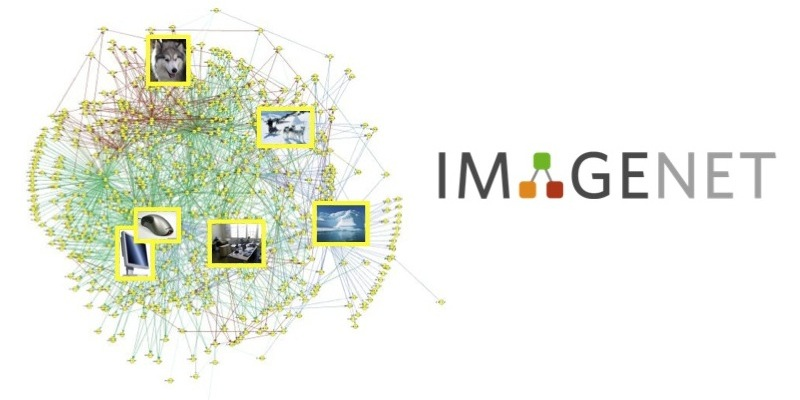
\includegraphics[width=7.5cm]{figures/imagenet.jpg}}
    {\centering Image from \url{http://web.eecs.umich.edu/~jiadeng/}}
\end{center}

\end{frame}

% -----------------------------------------------------------------------------

\begin{frame}[fragile]
\frametitle{Deep Learning}
\framesubtitle{Applications -- Object Classification and Localization}

CNNs have lead to significant performance gains on ImageNet % 2015 results not online yet

% check the website for more infos on the newest results and the DL architectures used
% basically it's smaller receptive fields and deeper architectures (up to 19 in case of the 2014 runner up, for around 140 million parameters)

% below errors are top-5 error percentages - result is regarded as correct if one out of five reported categories corresponds to the true label (because there are multiple objects in the images, causing ambiguity) in case of classification. for localization, the bounding box must be correct as well.

\bigskip
\begin{center}
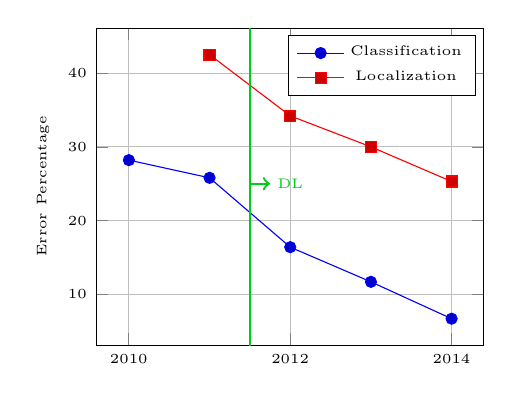
\begin{tikzpicture}
\begin{axis}[
    x tick label style={/pgf/number format/1000 sep=},
    ylabel=Error Percentage,
    font=\tiny,
    ylabel near ticks,
    grid=major
]
\addplot coordinates {(2010,28.2) (2011,25.8) (2012,16.4) (2013,11.7) (2014,6.7)};
\addplot coordinates {(2011,42.5) (2012,34.2) (2013,30.0) (2014,25.3)};
\draw [darkgreen,thick] (axis cs:2011.5,0) -- (axis cs:2011.5,50);
\draw [->,darkgreen,thick] (axis cs:2011.5,25) -- (axis cs:2011.75,25);
\node [darkgreen,thick] at (axis cs:2012,25) {DL};
\legend{Classification,Localization}
\end{axis}
\end{tikzpicture}
\end{center}

\end{frame}

% -----------------------------------------------------------------------------

\begin{frame}[fragile]
\frametitle{Deep Learning}
\framesubtitle{Applications -- Object Classification and Localization}

Demo of winner of 2013 ImageNet classification challenge

\bigskip
\begin{center}
    \copyrightbox[b]
    {
\includegraphics[width=7cm]{figures/clarifai.jpg}}
    {\centering Image from \href{http://www.clarifai.com}{\texttt{clarifai.com}}}
\end{center}

\end{frame}

% -----------------------------------------------------------------------------

\begin{frame}[fragile]
\frametitle{Deep Learning}
\framesubtitle{Applications -- Object Detection}

Results of 2014 ImageNet object detection challenge (excerpt) % see below slide for detection definition

% DL wins if there is much data available (no *), but a shallow method MUS won the competition on a reduced data set (*) to a deep method (MSRA). complex DL nets require a significant amount of training data due to the large number of parameters, which can be a limitation

\medskip
\begin{center}
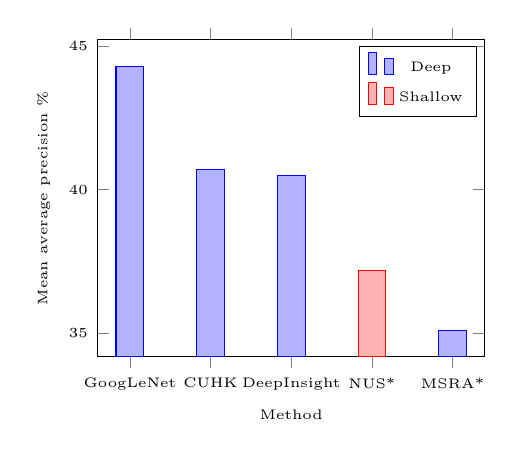
\begin{tikzpicture}
\begin{axis}[
    symbolic x coords={GoogLeNet,CUHK,DeepInsight,NUS*,MSRA*},
    xtick={GoogLeNet,CUHK,DeepInsight,NUS*,MSRA*},
    ybar,
    bar shift=0pt,
    font=\tiny,
    xlabel=Method,
    ylabel=Mean average precision \%
]
\addplot coordinates {(GoogLeNet,44.3) (CUHK,40.7) (DeepInsight,40.5) (MSRA*,35.11)};
\addplot coordinates {(NUS*,37.2)};
\legend{Deep,Shallow}
\end{axis}
\end{tikzpicture}
\end{center}

\end{frame}

% -----------------------------------------------------------------------------

\begin{frame}
\frametitle{Deep Learning}
\framesubtitle{Libraries and Resources}

Many open-source libraries available
\begin{itemize}
    \item Caffe (C++, Matlab, Python)
    \item Keras, Lasagne (Python)
    \item ConvNetJS (Java Script)
    \item Torch7 (LUA)
\end{itemize}

\bigskip
Network definitions and trained networks available online
\begin{itemize}
    \item E.g.\ Caffe model zoo
\end{itemize}

\end{frame}

% -----------------------------------------------------------------------------

\begin{frame}
\frametitle{Deep Learning}
\framesubtitle{Remarks}

Deep learning and CNNs are powerful concepts
\begin{itemize}
    \item State of the art in image recognition
\end{itemize}

\bigskip
Large CNNs have millions of parameters
\begin{itemize}
    \item Training takes long (up to weeks on GPUs)
    \item Requires large datasets to avoid overfitting
\end{itemize}

\end{frame}

% -----------------------------------------------------------------------------

\setstretch{1}
\renewcommand\emph[1]{\oldemph{#1}}

\begin{frame}[allowframebreaks=0.8]
\frametitle{Bibliography}

\printbibliography

\end{frame}

\end{document}
